\documentclass[aspectratio=169,11pt]{beamer}
\usepackage{teaching_slides}


\title [Single-agent dynamic optimization models]{Single-agent dynamic optimization models}
\author{C.Conlon - help from M. Shum and Paul Scott}
\institute{Grad IO }
\date{}
\setbeamerfont{equation}{size=\tiny}

\begin{document}
\begin{frame}
\titlepage
\end{frame}

\section{Rust Implementation}

\begin{frame}{Rust (1987)}
Likelihood function for a single bus:
\begin{equation*}
\begin{split}
& \ell (x_1, \cdots , x_T, d_1, \cdots , d_T | x_0, d_0 ; \theta) \\
= & \prod^T_{t=1} \Pr(d_t, x_t | x_0, d_0, \cdots , x_{t-1}, d_{t-1} ; \theta) \\
= & \prod^T_{t=1} \Pr(d_t, x_t |  x_{t-1}, d_{t-1} ; \theta) \\
= & \prod^T_{t=1} P(d_t | x_t; \theta) \cdot \prod^T_{t=1} f (x_t | x_{t-1}, d_{t-1} ; \theta^f) .
\end{split}
\end{equation*}
The third line arises from the Markovian feature of the problem, and the last equality arises due to the conditional independence assumption.
\end{frame}

\begin{frame}{Rust (1987)}
Log likelihood is additively separable in the two components:
\begin{equation*}
\text{log } \ell(\theta) = \sum^T_{t=1} \text{log } P (d_t | x_t ; \theta) + \sum^T_{t=1} \text{log } f (x_t | x_{t-1}, d_{t-1}; \theta^f).
\end{equation*}
Given the factorization of the likelihood function above, we can estimate in two steps... \\
\vspace{3mm}
\end{frame}

\begin{frame}{Step 1: Estimate Markov TPM}
\footnotesize
\begin{itemize}
\item Estimate $\theta^f$, the parameters of the Markov transition probabilities for mileage, conditional on non-replacement of engine (i.e. $d_t = 0$)
\item Recall that a replacement resets mileage to zero: if $d_t = 1$, then $x_{t+1} = 0 + \Delta_{t+1}$
\end{itemize}

We assume a discrete distribution for $\Delta_{t+1} \equiv x_{t+1} - x_t$ (when $d_t = 0$), the incremental mileage between any two periods:
\begin{align*}
\Delta_{t+1} = \left \{
\begin{matrix}
[0, 5000) & \text{w/prob } \theta^f_0 \\
[5000, 10000) & \text{w/prob } \theta^f_1 \\
[10000, \infty) & \text{w/prob } 1 - \theta^f_0 - \theta^f_1
\end{matrix}
\right .
\end{align*}
so that $\theta^f \equiv \{\theta^f_0, \theta^f_1 \}$, with $0 < \theta^f_0, \theta^f_1< 1$ and $\theta^f_0 + \theta^f_1 < 1$. \\
\vspace{2mm}
\begin{itemize}
\item $\hat \theta^f$ estimated by empirical frequencies: $\hat \theta^f_0 = \text{freq} \{ \Delta_{t+1} \in  [0, 5000) \}$, etc.
\item Note: this does not require the behavioral model!
\end{itemize}
\end{frame}

\begin{frame}{Step \#2: Estimate Structural Parameters of Cost Function}
\footnotesize
Start by treating $(\beta, \hat \theta^f)$ as given:
\begin{enumerate}
\item Fix a guess of $(RC,\theta^c)$ the remaining parameters.
\item Iterate on the Bellman Operator for $(\beta,\theta^c,\theta^f,RC)$ using \alert{Value Function Iteration} to get $V^*(x,\varepsilon)$ or $v^*(x,d)$.
\item Calculate \alert{conditional choice probabilities} (CCPs):
\begin{align*}
P(d_t=1 | x_t;\theta) &=  \frac {\exp[ v_{\theta} (x_t, 1)]  }{\exp[v_{\theta} (x_t, 0)] + \exp[ v_{\theta} (x_t, 1)]}
\end{align*}
\item Evaluate the log-likelihood:
\begin{align*}
\ell(\theta) = \sum^T_{t=1} \log P (d_t | x_t ; \theta^c,RC, \hat{\theta}^f) + \underbrace{\sum^T_{t=1} \log f (x_t | x_{t-1}, d_{t-1}; \hat{\theta}^f)}_{\text{Can Ignore! Why?}}
\end{align*}
\end{enumerate}
Solve via MLE. This is the \alert{Nested Fixed Point} algorithm.
\end{frame}

\begin{frame}{Computational Details}
That looked easy, except that I never really showed you how to recover $v_{\theta}(x,d)$:
\begin{itemize}
\item Directly iterating on Bellman's operator requires keeping track of $\varepsilon$'s which are: (1) unobserved to you the econometrician and (2) continuous and full support (not a discrete grid).
\begin{itemize}
\item AKA a big pain.
\end{itemize}
\item You may (or may not) have learned some tricks for solving Bellman equations in Macro that you could apply here: VFI, Policy Iteration (PI), Howard's Policy Improvement, etc.
\begin{itemize}
\item None of that really tells us how to deal with $\varepsilon$'s.
\end{itemize}
\end{itemize}
\end{frame}

\begin{frame}{Rust's Trick}\

\begin{itemize}
\item Rust has a nice trick that lets us work with a new function $EV_{\theta}(x,d)$ instead of $V_{\theta}(x,\varepsilon)$ we call this the \alert{expected value function}.
\begin{eqnarray*}
EV(x, d) \equiv \E_{x', \varepsilon ' | x, d} V(x', \varepsilon ' ; \theta)
\end{eqnarray*}
\item In words $EV_{\theta}(x,d)$ says at time $t-1$ what is the expected value of $V_{\theta}(x_t,\varepsilon_t)$ [eq 4.14].
\begin{align*}
EV(x,d) = \int_y \log \left \{ \sum_{d' \in C(y)} \exp [ u(y,d'; \theta) + \beta EV(y, d')] \right \} f(dy|x,d)
\end{align*}
\item Here $x, d$ denotes the \emph{previous} period's mileage and replacement choice, and $y, d'$ denote the \emph{current} period's mileage and choice.
\end{itemize}
\end{frame}

\begin{frame}{Derivation of Rust's Trick}
\footnotesize
This \alert{expected value function} can be derived from Bellman's equation:
\begin{align*}
\begin{split}
V(y, \varepsilon ;\theta) = & \max_{d' \in 0,1} [ u(y, d' ; \theta) + \varepsilon(d') + \beta EV(y,d')] \\
\Longrightarrow & \E_{y, \varepsilon} [V(y, \varepsilon ; \theta) | x, d ] \equiv  EV(x, d ; \theta) \\
= & \E_{y, \varepsilon | x, d } \left \{ \max_{ d' \in 0,1} [ u(y, d' ; \theta) + \varepsilon(d') + \beta EV(y,d')] \right \} \\
= &  \E_{y | x, d }  \E_{\varepsilon | y } \left \{ \max_{ d' \in 0,1} [ u(y, d' ; \theta) + \varepsilon(d') + \beta EV(y,d')] \right \} \\
= &  \E_{y | x, d } \log \left \{ \sum_{d'=0,1} \exp [ u(y, d' ; \theta)  + \beta EV(y,d')] \right \} \\
= & \int_y \log  \left \{ \sum_{d'=0,1} \exp [ u(y, d' ; \theta)  + \beta EV(y,d')] \right \} f(dy|x,d).
\end{split}
\end{align*}
The fourth line drops Euler's $\gamma$ from $\E \max$: keeping it adds $\gamma/(1-\beta)$ to every $EV(x,d)$ and leaves the CCPs unchanged.
\end{frame}
%
%\begin{frame}{Rust (1987)}
%The next-to-last equality uses the closed-form expression for the expectation of the maximum, for extreme-value variates.\\
%\vspace{3mm}
%Once the $EV(x, i ;\theta)$ function is computed for $\theta$, the choice probabilities $p(i_t |x_t)$ can be constructed as
%\begin{equation*}
%\frac {\exp(u(x_t, i_t ;\theta) + \beta EV (x_t, i_t; \theta))}{\sum_{i=0,1} \exp(u(x_t, i;\theta) + \beta EV(x_t, i;\theta))}.
%\end{equation*}
%\end{frame}

\begin{frame}{In Rust's model: one value function on the grid}
\footnotesize
\begin{itemize}
\item Standard timing gives $f(x' \mid x, 1) = f(x' \mid 0, 0)$, so replacing at $x$ has the same continuation value as keeping at $0$:
\begin{align*}
EV(x,1) = EV(0,0) \qquad \Longrightarrow \qquad \text{write } EV(x) \equiv EV(x,0)
\end{align*}
\item The two choice-specific values on a grid of $N$ mileage states:
\begin{align*}
v(x,0) &= -c(x;\theta^c) + \beta\, EV(x)\\
v(x,1) &= -RC - c(0;\theta^c) + \beta\, EV(0) \qquad \text{(constant in } x\text{)}
\end{align*}
\item CCP:
\begin{align*}
P(1 \mid x;\theta) = \frac{1}{1 + \exp\left[v(x,0) - v(x,1)\right]}
\end{align*}
\item Bellman equation: one $N$-vector fixed point,
\begin{align*}
EV(x) = \sum_{x'} f(x' \mid x, 0;\theta^f)\, \ln \left[ e^{v(x',0)} + e^{v(x',1)} \right], \qquad \text{i.e. } EV = \symbf{F}_0 \ln\left(e^{v_0} + e^{v_1}\right)
\end{align*}
where $\symbf{F}_0$ is the keep transition matrix (rows = current state) and $v_d$ stacks $v(x,d)$ over $x$.
\end{itemize}
\end{frame}

\begin{frame}{Value Function Iteration}
\footnotesize
\begin{enumerate}
\item Start with an initial guess at $k=0$ for $EV^{k}_{\theta}(x,d)$. A common guess is $EV_{\theta}^{0}(x,d) = 0$ for all $(x,d)$
\item Iterate Bellman Operator
\begin{align*}
T_{\theta}\left(EV_{\theta}^{k}\right)= & \int_y \log  \left \{ \sum_{d'=0,1} \exp [ u(y, d' ; \theta)  + \beta EV^{k}(y,d')] \right \} f(dy|x,d).
\end{align*}
with $f(dy | x, d; \hat \theta^f)$ estimated in Step 1.\\

$T_{\theta}\left(EV_{\theta}^{k}(x,d)\right)\equiv EV_{\theta}^{k+1}(x,d)$.\\
\item Compare $\epsilon(k) \equiv \sup_{(x,d)} | EV_{\theta}^{k+1}(x,d) - EV_{\theta}^{k}(x,d)|$ to $\epsilon^{tol}$. If $\epsilon(k) \leq \epsilon^{tol}$ then stop.
\end{enumerate}
See my notes on Numerical Dynamic Programming for more details.
\end{frame}

\begin{frame}{Solving the fixed point}
Obvious approach is contraction iterations (VFI):
\begin{align*}
E V_{\theta}^{k}=T_{\theta}\left(E V_{\theta}^{k-1}\right)=T_{\theta}^{k}\left(E V_{0}\right)
\end{align*}
Rust actually switches to Newton-Kantorovich Iteration:
\begin{align*}
E V_{\theta}^{k+1}=E V_{\theta}^{k}-\left[I-T_{\theta}^{\prime}\right]^{-1}\left(I-T_{\theta}\right)\left(E V_{\theta}^{k}\right)
\end{align*}
The first is slow, but globally convergent. The second is fast but locally convergent. To get the gradient of the log-likelihood we must also calculate the Jacobian using the IFT:
\begin{align*}
\partial E V_{\theta} / \partial \theta=\left[I-T_{\theta}^{\prime}\right]^{-1} \partial T_{\theta}\left(E V_{\theta}\right) / \partial \theta
\end{align*}
See \url{https://editorialexpress.com/jrust/nfxp.pdf} for more details.
\end{frame}

\begin{frame}{Gradients: the implicit function theorem}
\footnotesize
\begin{itemize}
\item With $c(x;\theta^c) = \theta^c_1 x + \theta^c_2 x^2$, $\theta = (\theta^c_1, \theta^c_2, RC)$ and $EV(x) \equiv EV(x,0)$, the score is a logit score in the value difference:
\begin{align*}
\frac{\partial \ell}{\partial \theta} &= \sum_{i,t} \left[d_{it} - P(1 \mid x_{it};\theta)\right] \frac{\partial \left[v(x_{it},1) - v(x_{it},0)\right]}{\partial \theta}\\
\frac{\partial \left[v(x,1) - v(x,0)\right]}{\partial \theta} &= (x, x^2, -1)' + \beta \left[\frac{\partial EV(0)}{\partial \theta} - \frac{\partial EV(x)}{\partial \theta}\right]
\end{align*}
\item $EV$ solves $EV = T_\theta(EV)$, so by the IFT
\begin{align*}
\frac{\partial EV}{\partial \theta} &= \left[\symbf{I} - \frac{\partial T_\theta}{\partial EV}\right]^{-1} \frac{\partial T_\theta}{\partial \theta}, &
\frac{\partial T_\theta}{\partial EV} &= \beta\, \symbf{F}_0 \left[\mathrm{diag}\left(P(0 \mid \cdot)\right) + P(1 \mid \cdot)\, e_0' \right]
\end{align*}
and $\partial T_\theta/\partial \theta = -\symbf{F}_0 \left[ P(0\mid\cdot) \circ (x, x^2, 0) + P(1 \mid \cdot) \circ (0,0,1) \right]$.
\item Same matrix $\symbf{I} - \partial T_\theta/\partial EV$ as the Newton--Kantorovich step: one more linear solve.
\item Modern practice: automatic differentiation plus \alert{implicit differentiation} of the fixed point (e.g.\ \texttt{jax.lax.custom\_root}). Never differentiate through the iterations: slow, memory-hungry, and only as accurate as the inner tolerance.
\end{itemize}
\end{frame}



\begin{frame}{Value Function Iteration: Bounds}
\begin{itemize}
\item Suppose we set $V_0 =0$ then the value function iteration approach is just like solving the finite horizon problem by backward induction.
\item The CMT guarantees consistency at a geometric rate or \alert{linear} convergence with modulus $\beta$
\item We can derive an expression for the number of steps we need to get an $\epsilon$-approximation.
\begin{eqnarray*}
T(\epsilon,\beta) = \frac{1}{| \log(\beta) | } \log \left (\frac{1}{(1-\beta)\epsilon} \right)
\end{eqnarray*}
\item This tells us that when $\beta \rightarrow 1$ that VFI gets very very slow.
\end{itemize}
\end{frame}



\begin{frame}{Estimates}
\begin{center}
\hspace*{-.5cm}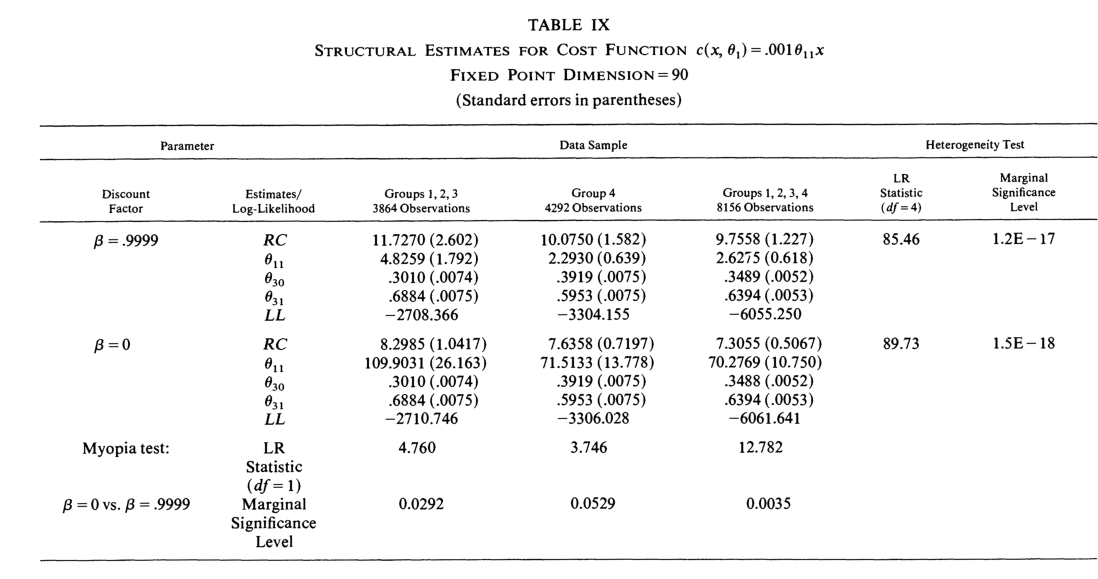
\includegraphics[scale=.58]{./resources/RustT9.pdf}
\end{center}
{\footnotesize Rust's notation: his $\theta_1$ (e.g.\ $\theta_{11}$) is our $\theta^c$, his $\theta_3$ (e.g.\ $\theta_{30}, \theta_{31}$) is our $\theta^f$, and his decision $i$ is our $d$.}
\end{frame}

\begin{frame}{Discount factor}
\begin{itemize}
	\item While Rust finds a better fit for $\beta=.9999$ than $\beta=0$, he finds that high levels
	of $\beta$ basically lead to the same level of the likelihood function.

	\medskip
	\item Furthermore, the discount factor is non-parametrically non-identified. Note:
	He loses ability to reject $\beta=0$ for more flexible cost function specifications.

\end{itemize}
\end{frame}


\begin{frame}{Discount factor {\footnotesize (Rust's $c(x,\theta_1)$ is our $c(x;\theta^c)$)}}
\begin{center}
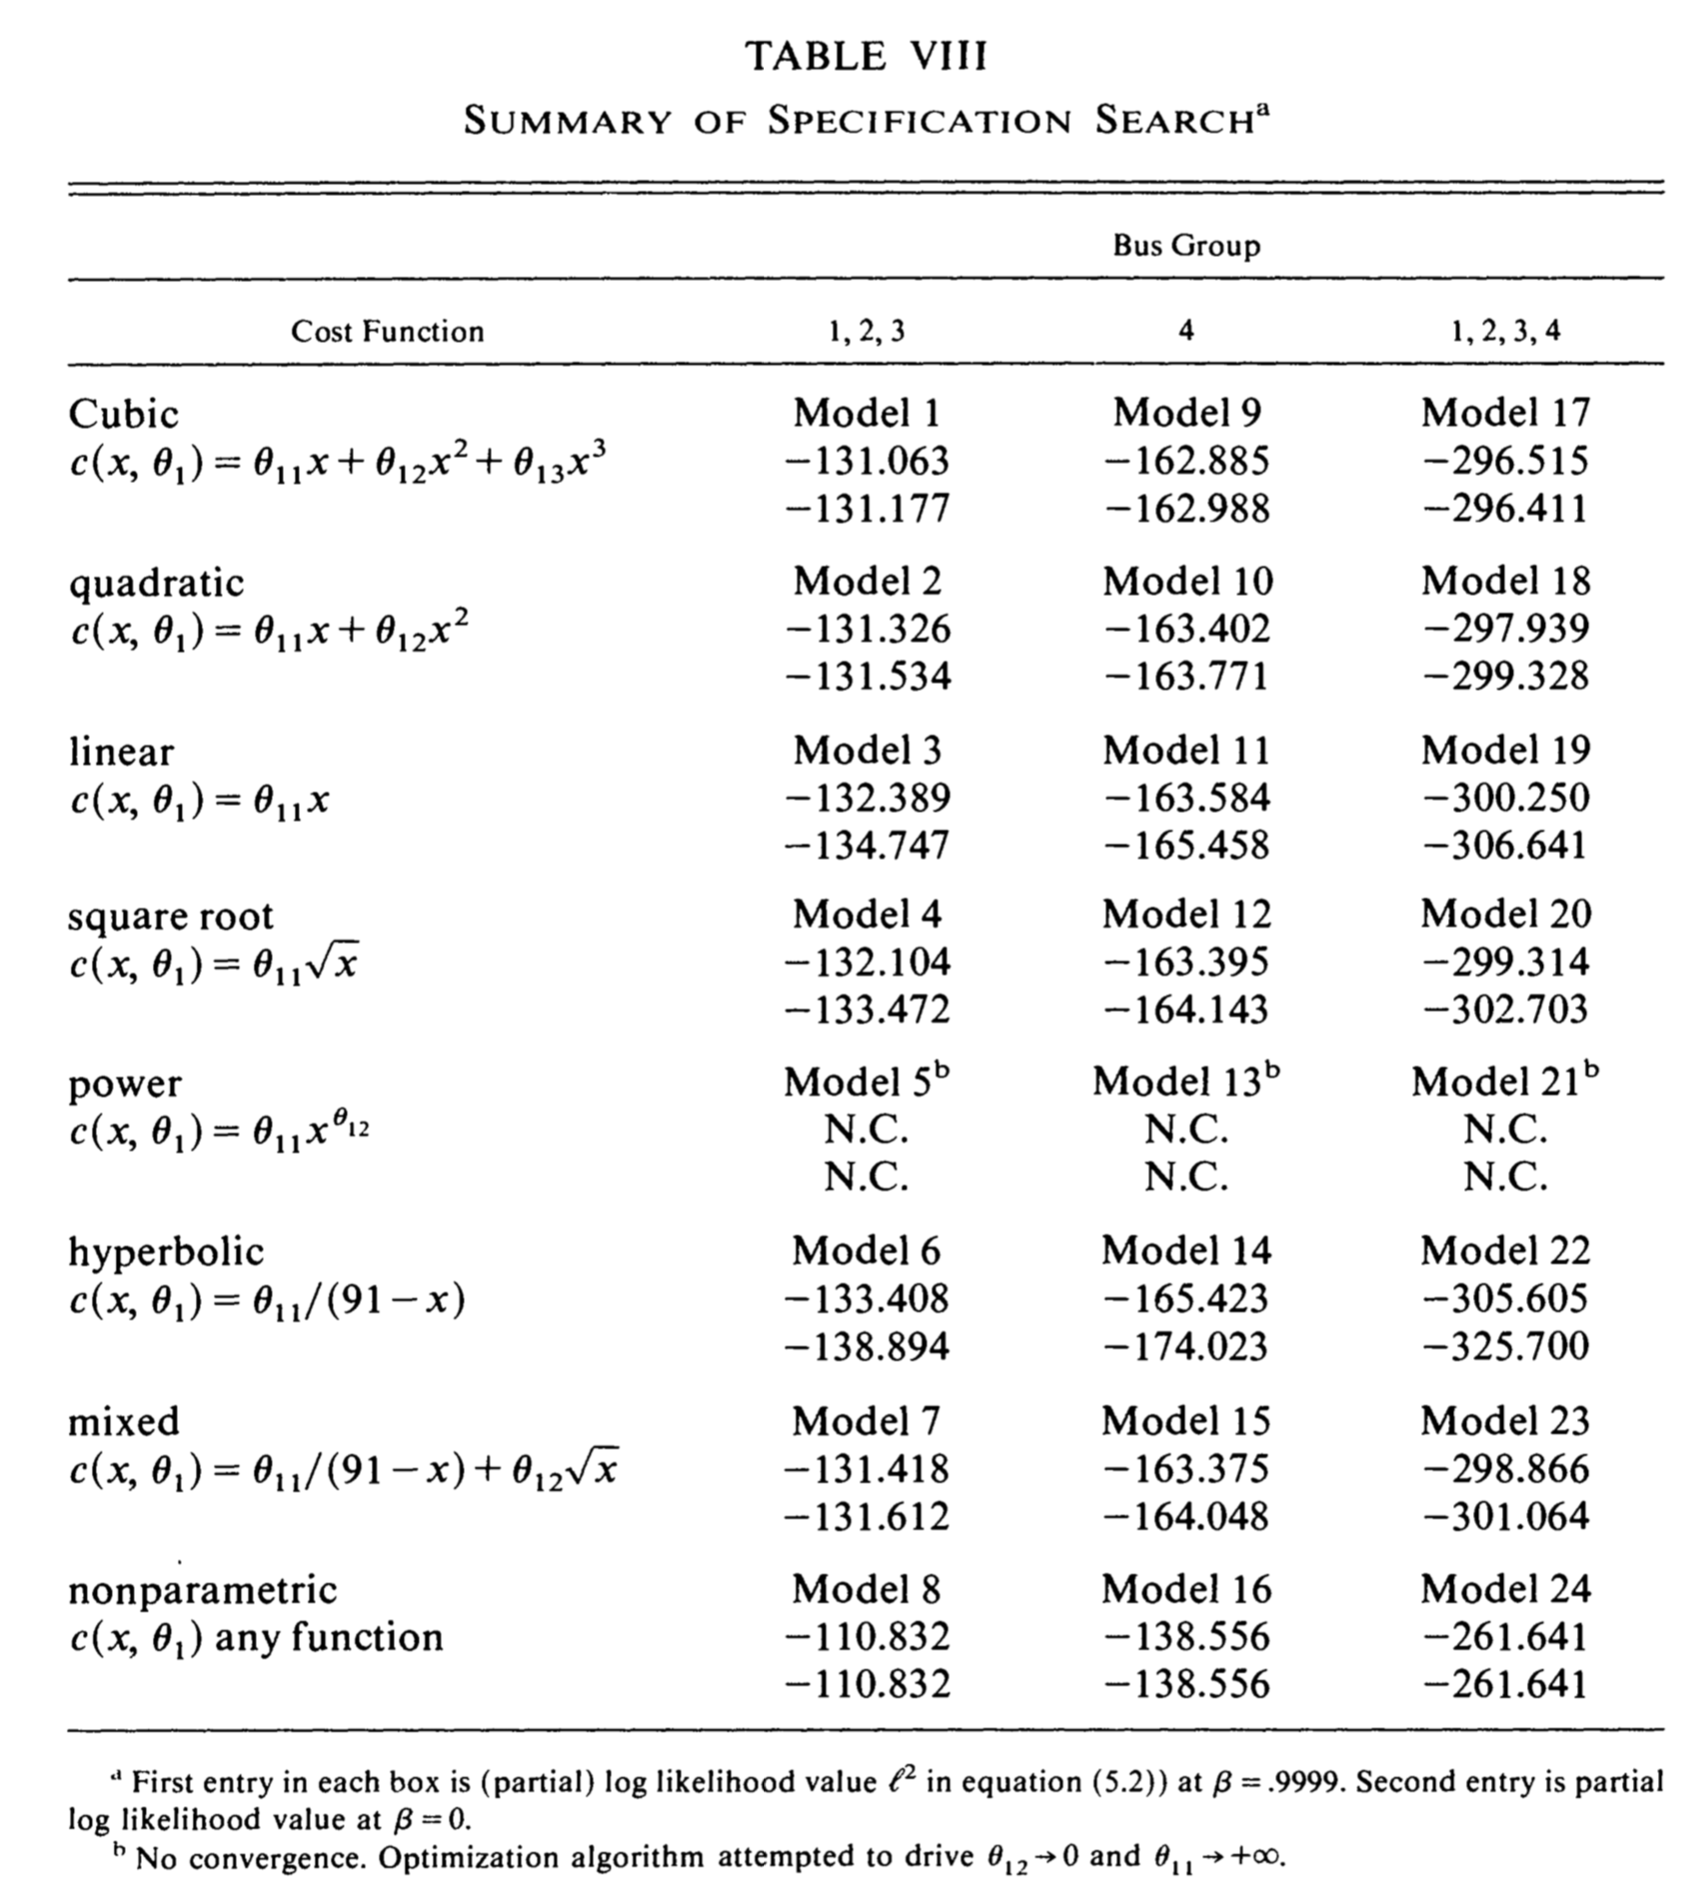
\includegraphics[scale=.25]{./resources/RustT8.png}
\end{center}
\end{frame}

\begin{frame}{Application}
\begin{center}
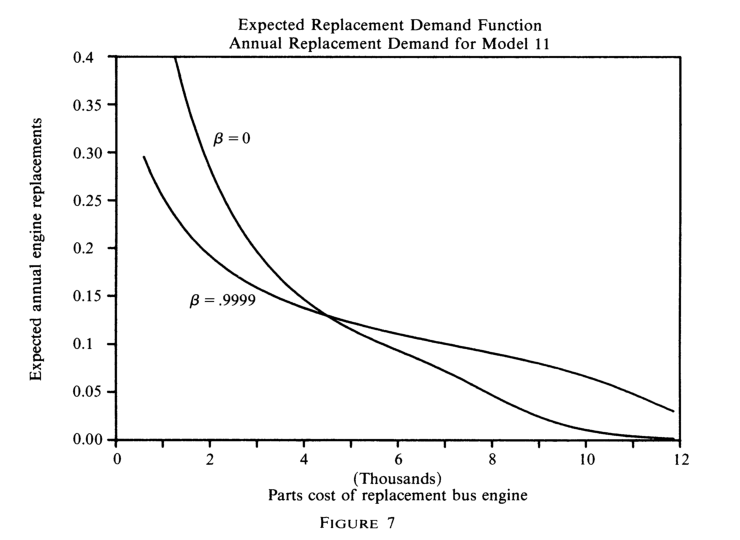
\includegraphics[scale=.8]{./resources/RustF7.pdf}
\end{center}
\end{frame}


\section{Thanks!}

\end{document}
